%----------------------------------------------------------------------------
\appendix
%----------------------------------------------------------------------------
\setcounter{chapter}{\appendixnumber}
%\setcounter{equation}{0} % a fofejezet-szamlalo az angol ABC 6. betuje (F) lesz
\numberwithin{equation}{section}
\numberwithin{figure}{section}
\numberwithin{lstlisting}{section}
%\numberwithin{tabular}{section}

\chapter{Heatmap designs}

\stepcounter{section}
\begin{figure}[!h]
    \centering
    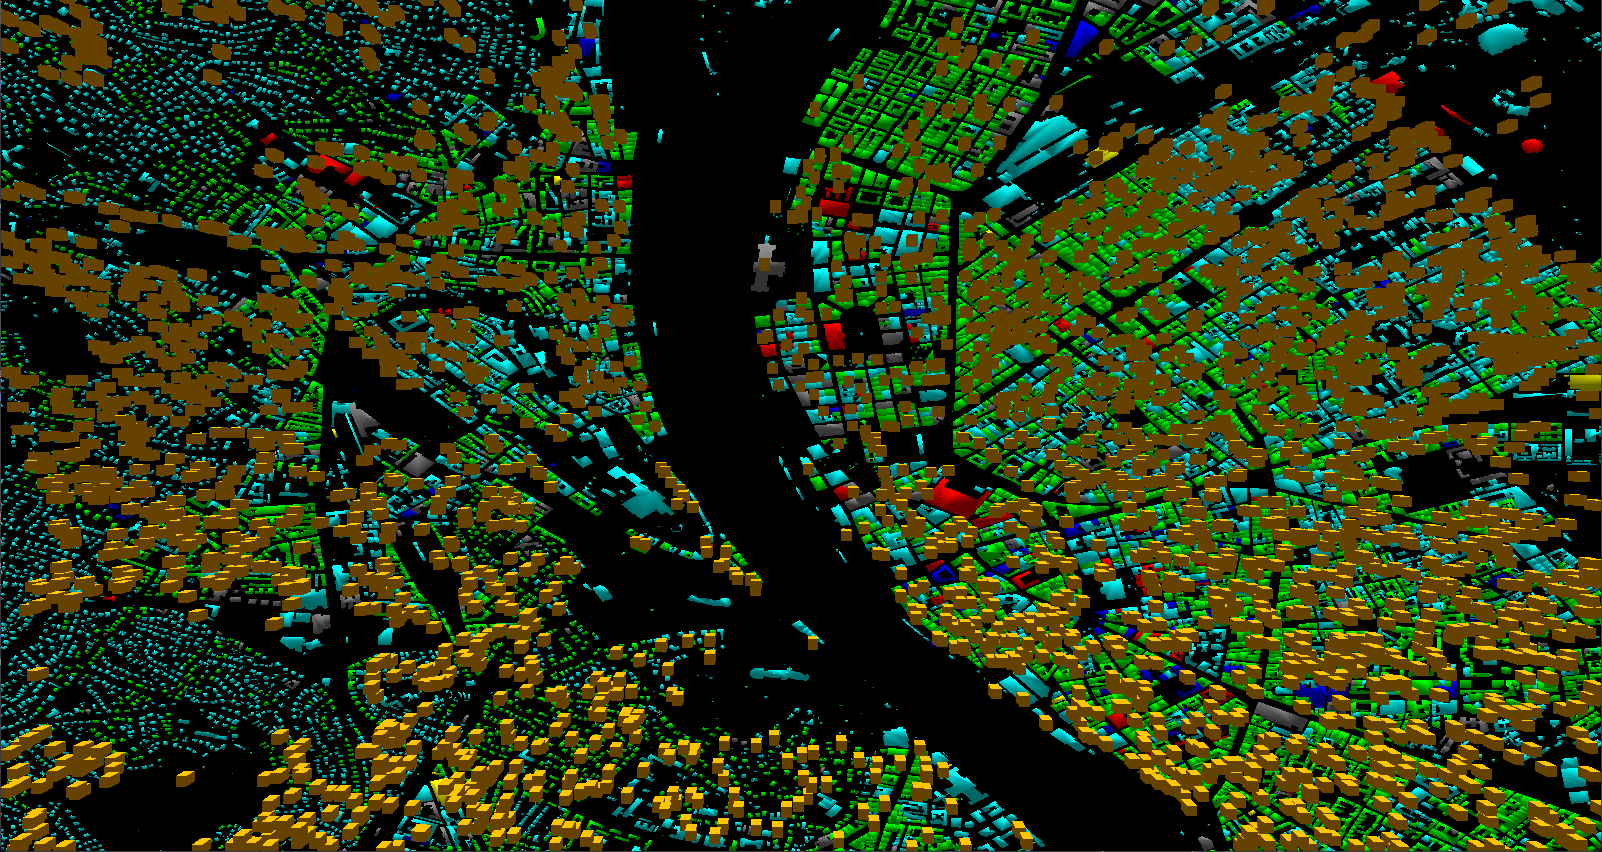
\includegraphics[width=110mm, keepaspectratio]{images/overlay_v1.png}
    \caption{An array of cubes displayed over the city of Budapest, each representing an agent; this was the first overlay version\ \label{overlay_v1}}
\end{figure}
\begin{figure}[!h]
    \centering
    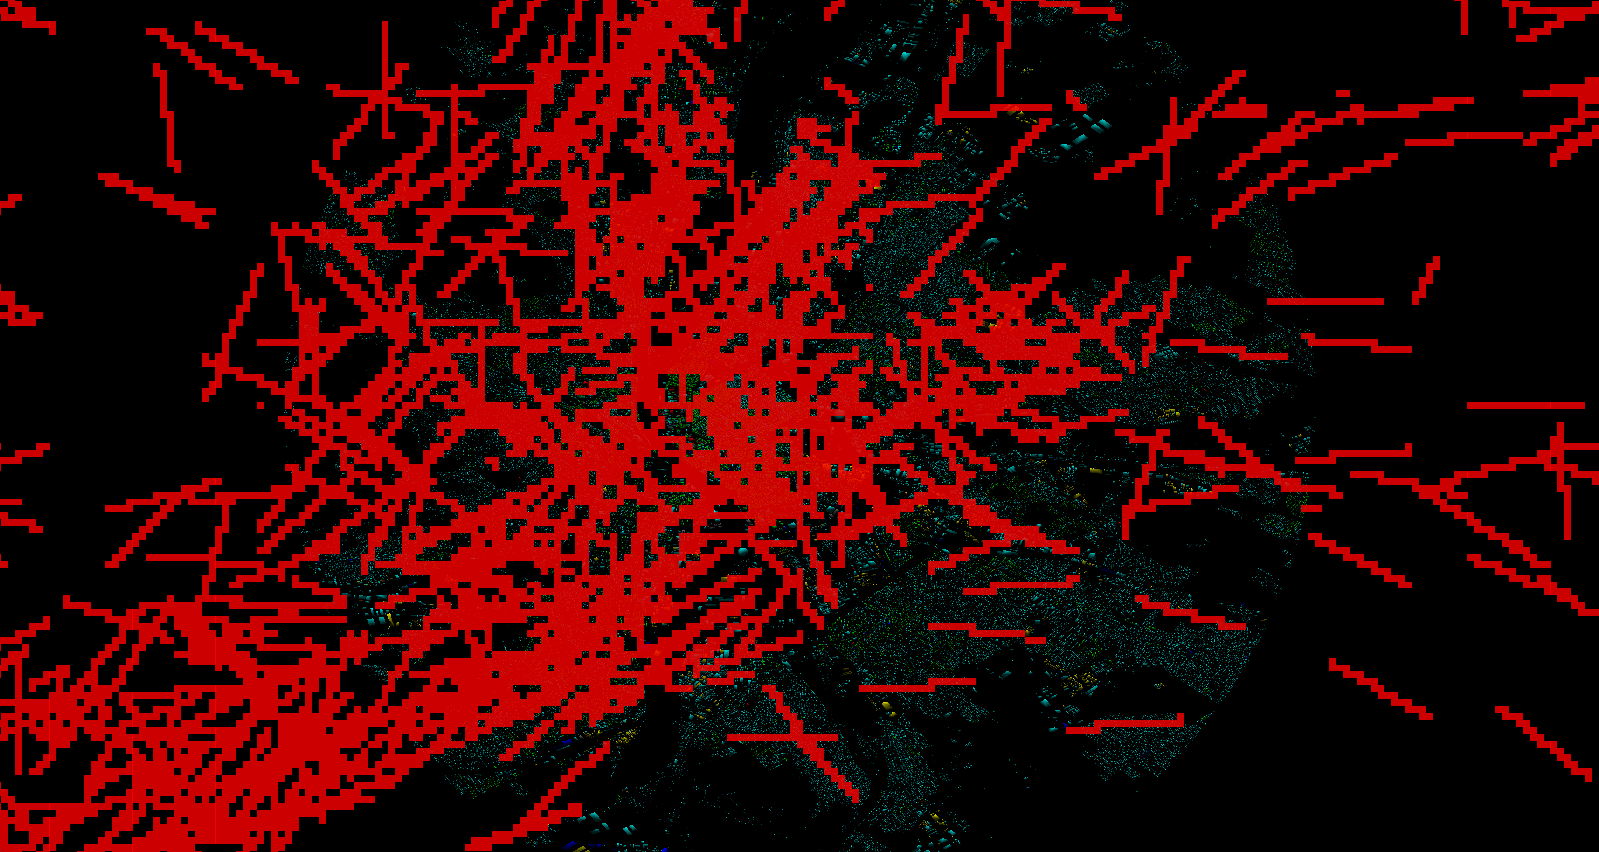
\includegraphics[width=110mm, keepaspectratio]{images/overlay_v2.png}
    \caption{An overlay with flattened opacity, displayed over the city of Budapest. Agent paths are randomised and are traversed in a straight line; this was the second overlay version\ \label{overlay_v2}}
\end{figure}

\label{comparison_heatmap}
\chapter{Agent count and age group comparison}

\stepcounter{section}
\begin{figure}[!h]
    \centering
    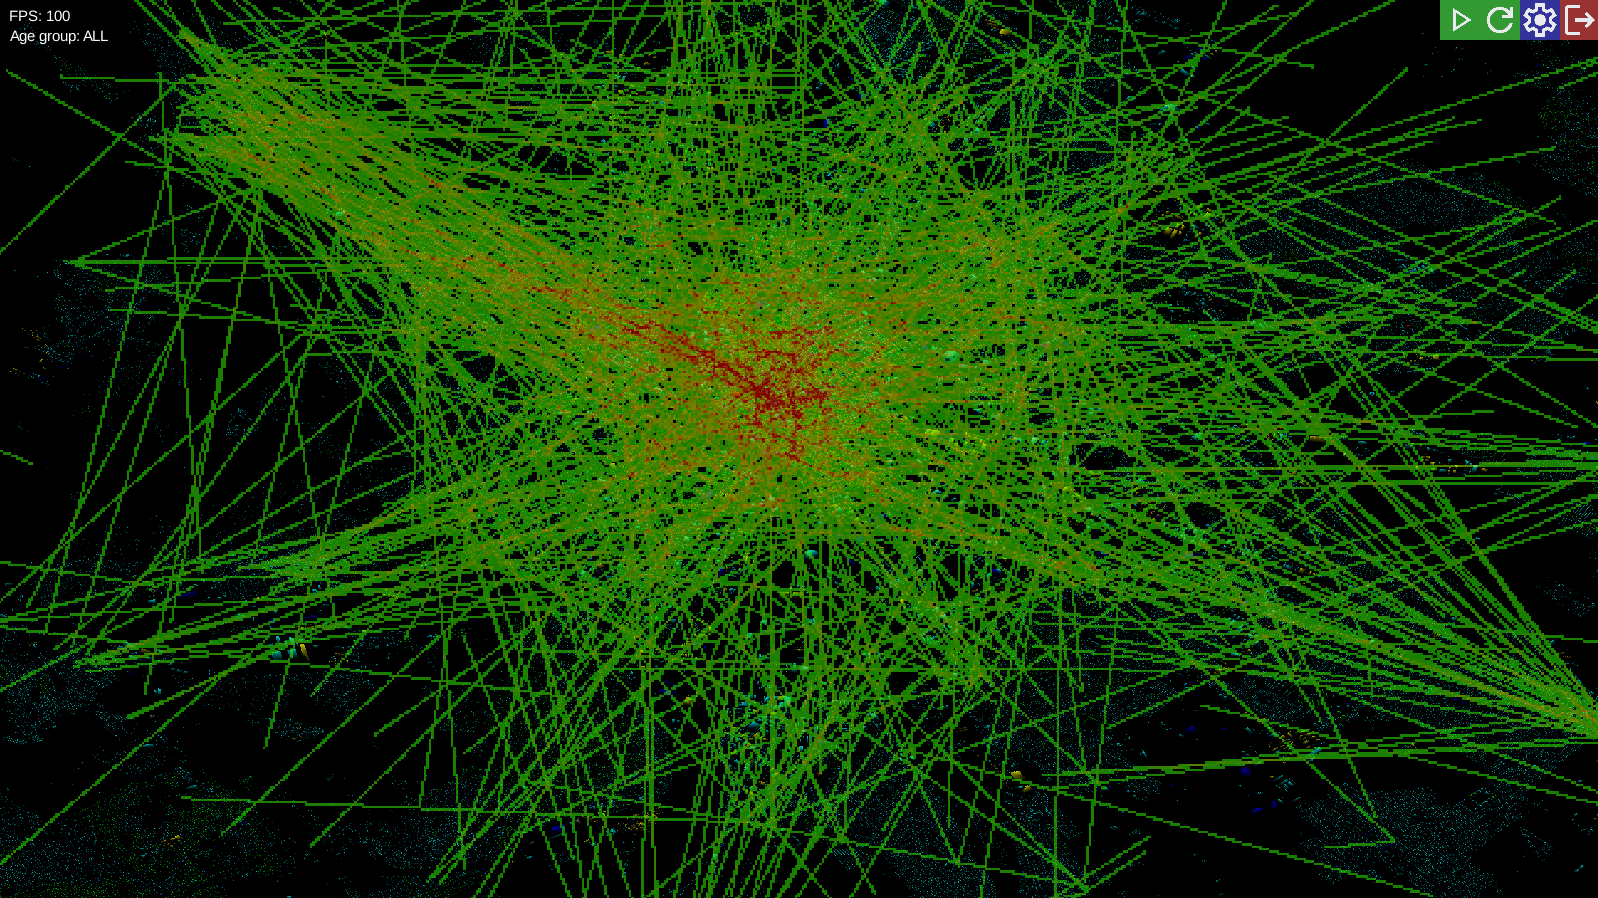
\includegraphics[width=110mm, keepaspectratio]{images/heatmap_1000.png}
    \caption{Heatmap using 1000 agents, see~\ref{perftesting-heatmap}}
\end{figure}
\begin{figure}[!h]
    \centering
    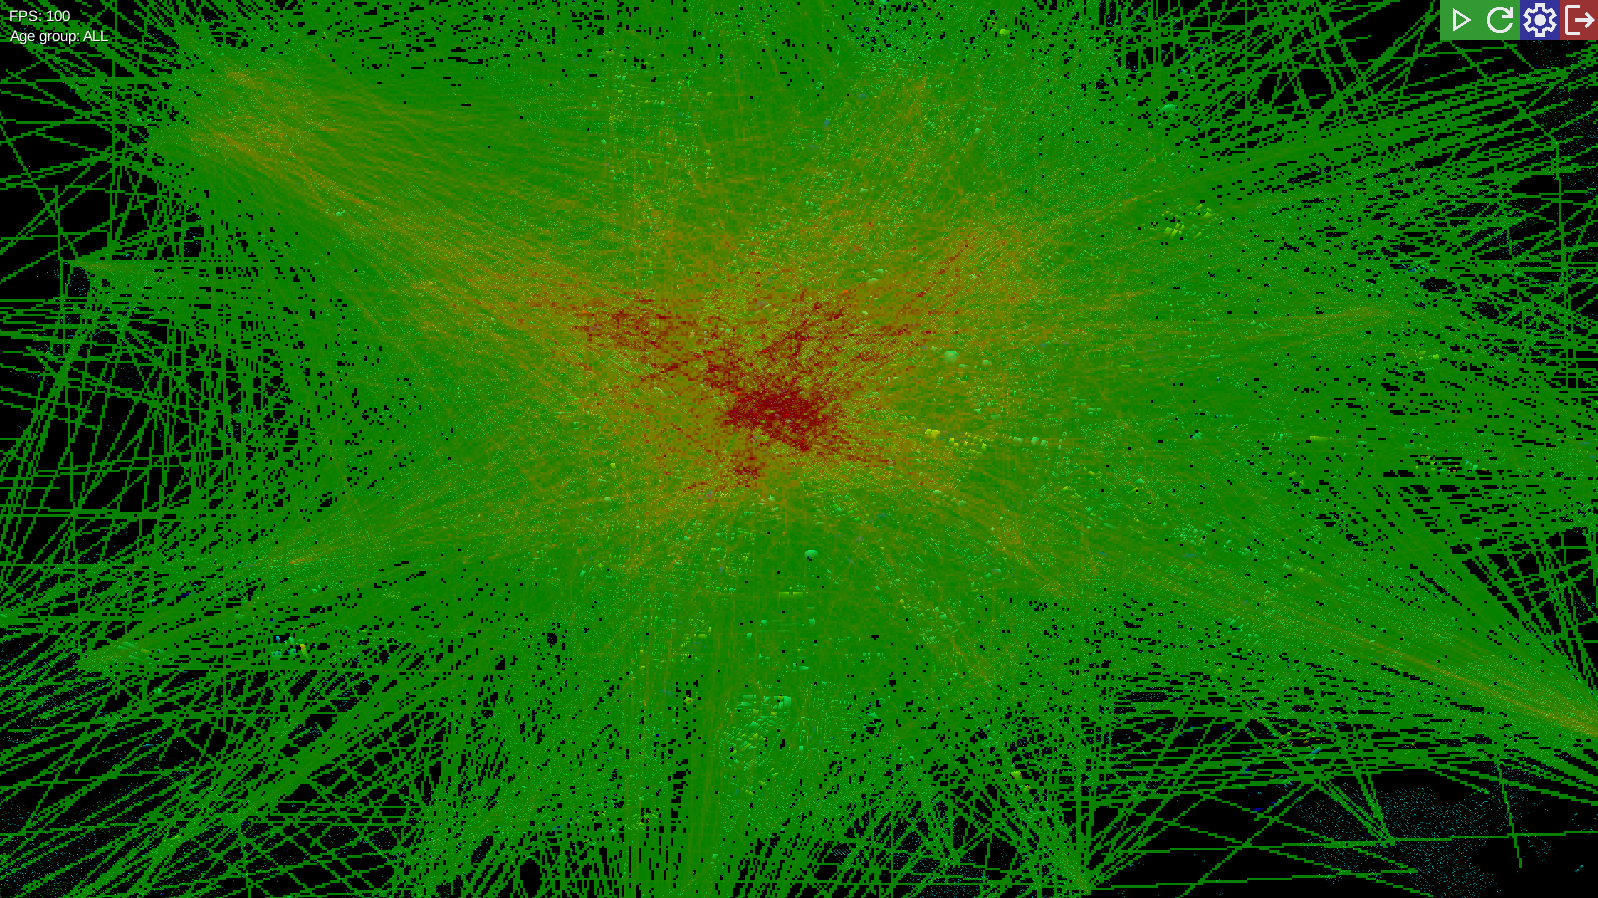
\includegraphics[width=110mm, keepaspectratio]{images/heatmap_5000.png}
    \caption{Heatmap using 5000 agents, see~\ref{perftesting-heatmap}}
\end{figure}
\begin{figure}[!h]
    \centering
    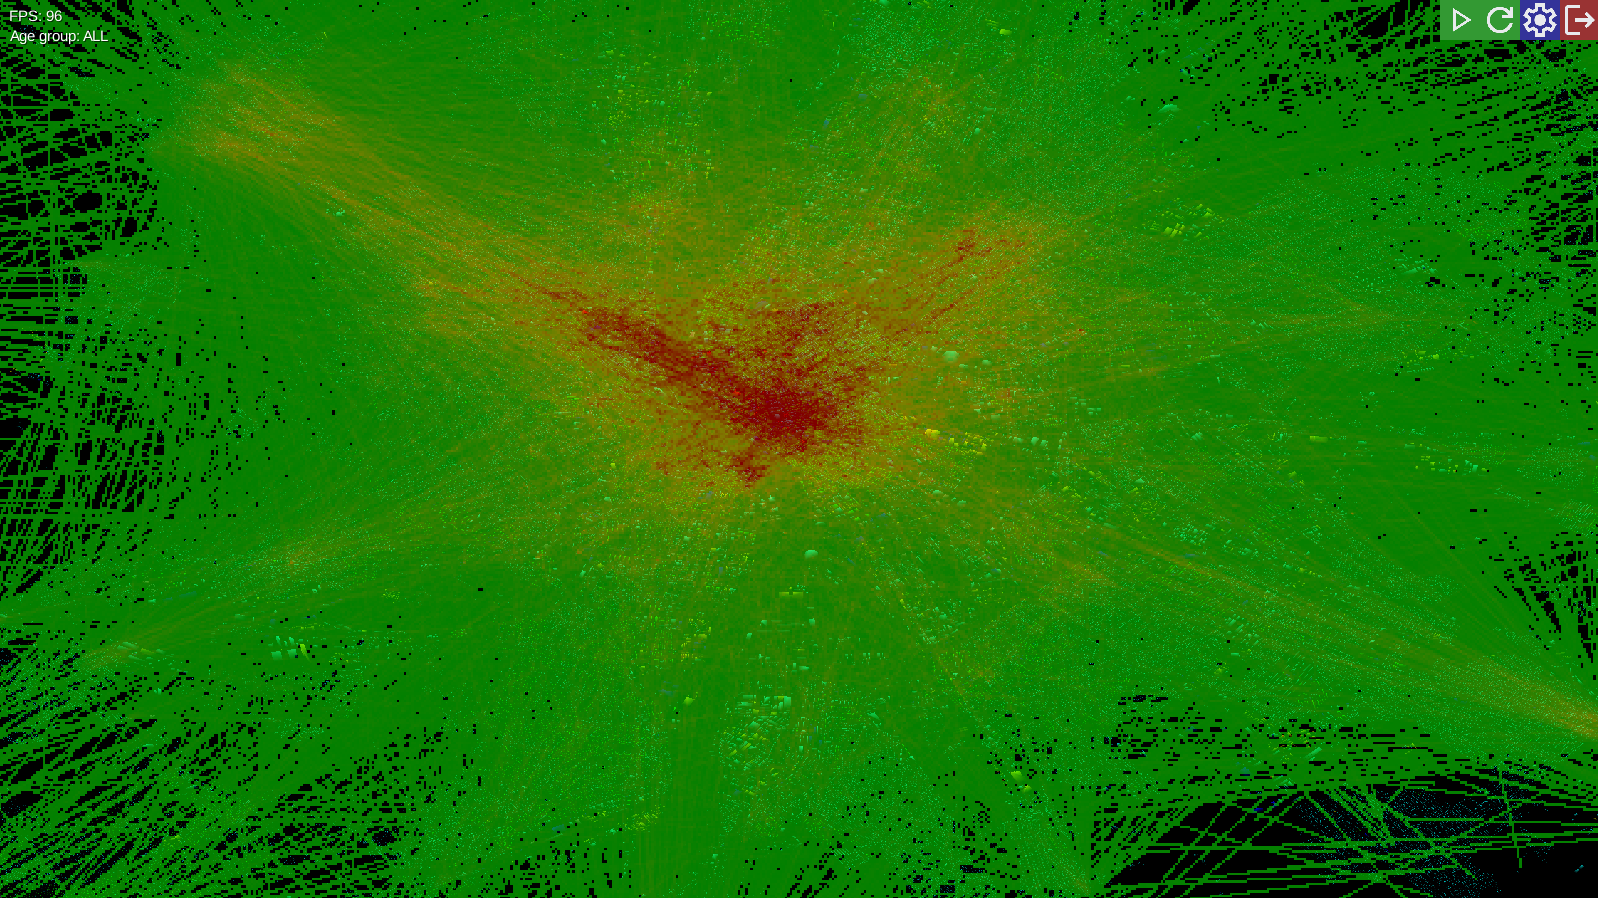
\includegraphics[width=110mm, keepaspectratio]{images/heatmap_10000.png}
    \caption{Heatmap using 10000 agents, see~\ref{perftesting-heatmap}}
\end{figure}
\begin{figure}[!h]
    \centering
    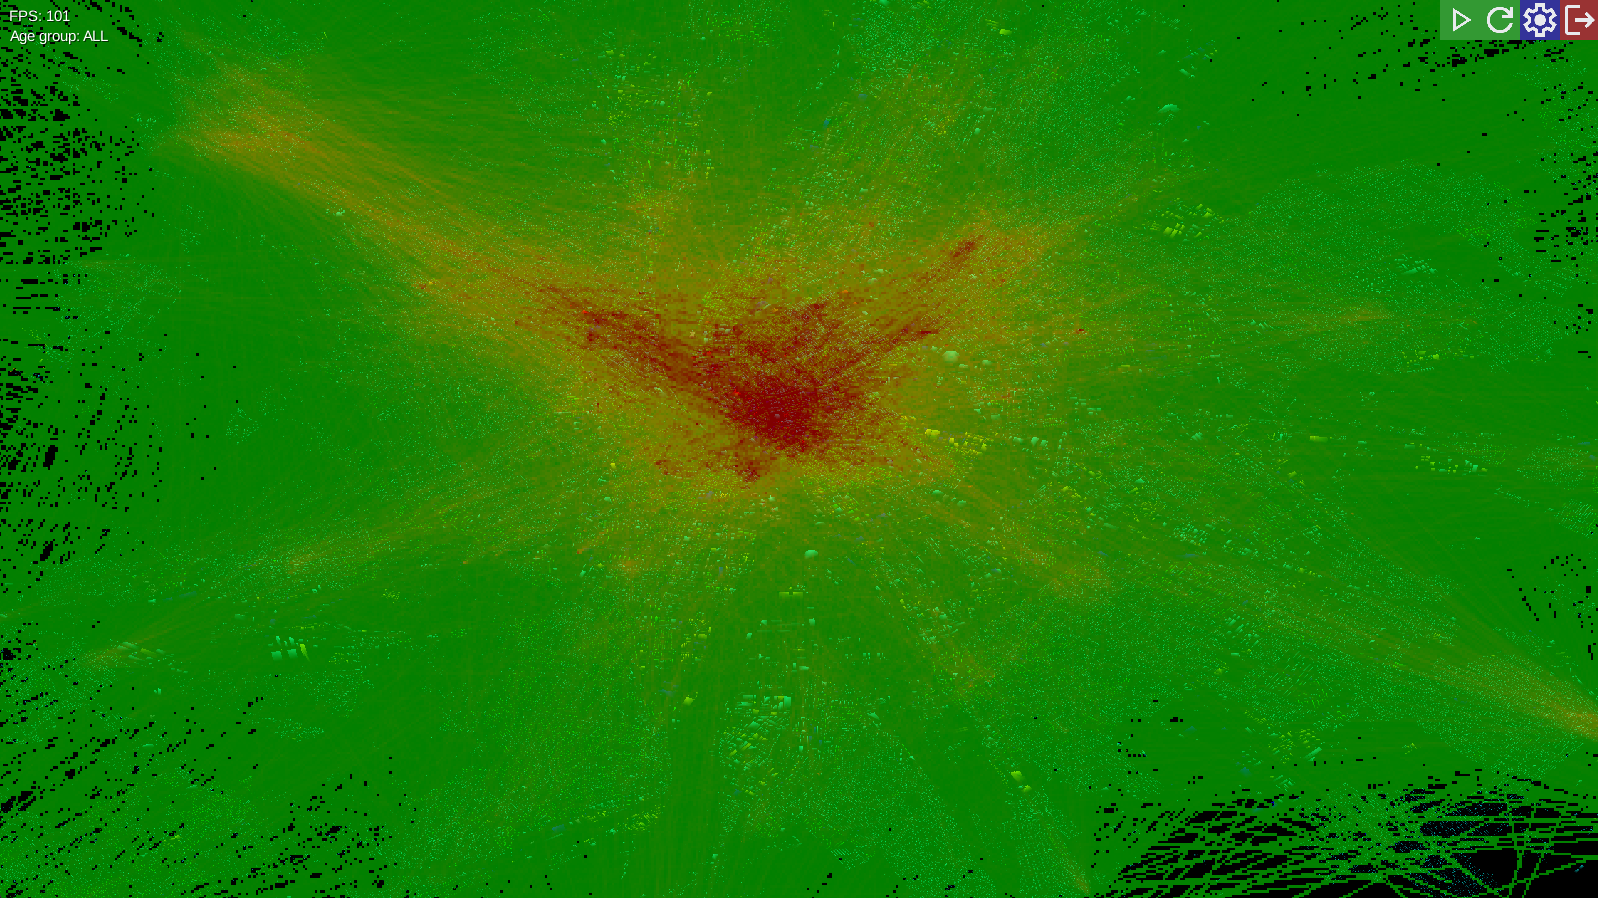
\includegraphics[width=110mm, keepaspectratio]{images/heatmap_20000.png}
    \caption{Heatmap using 20000 agents, see~\ref{perftesting-heatmap}}
\end{figure}
\begin{figure}[!h]
    \centering
    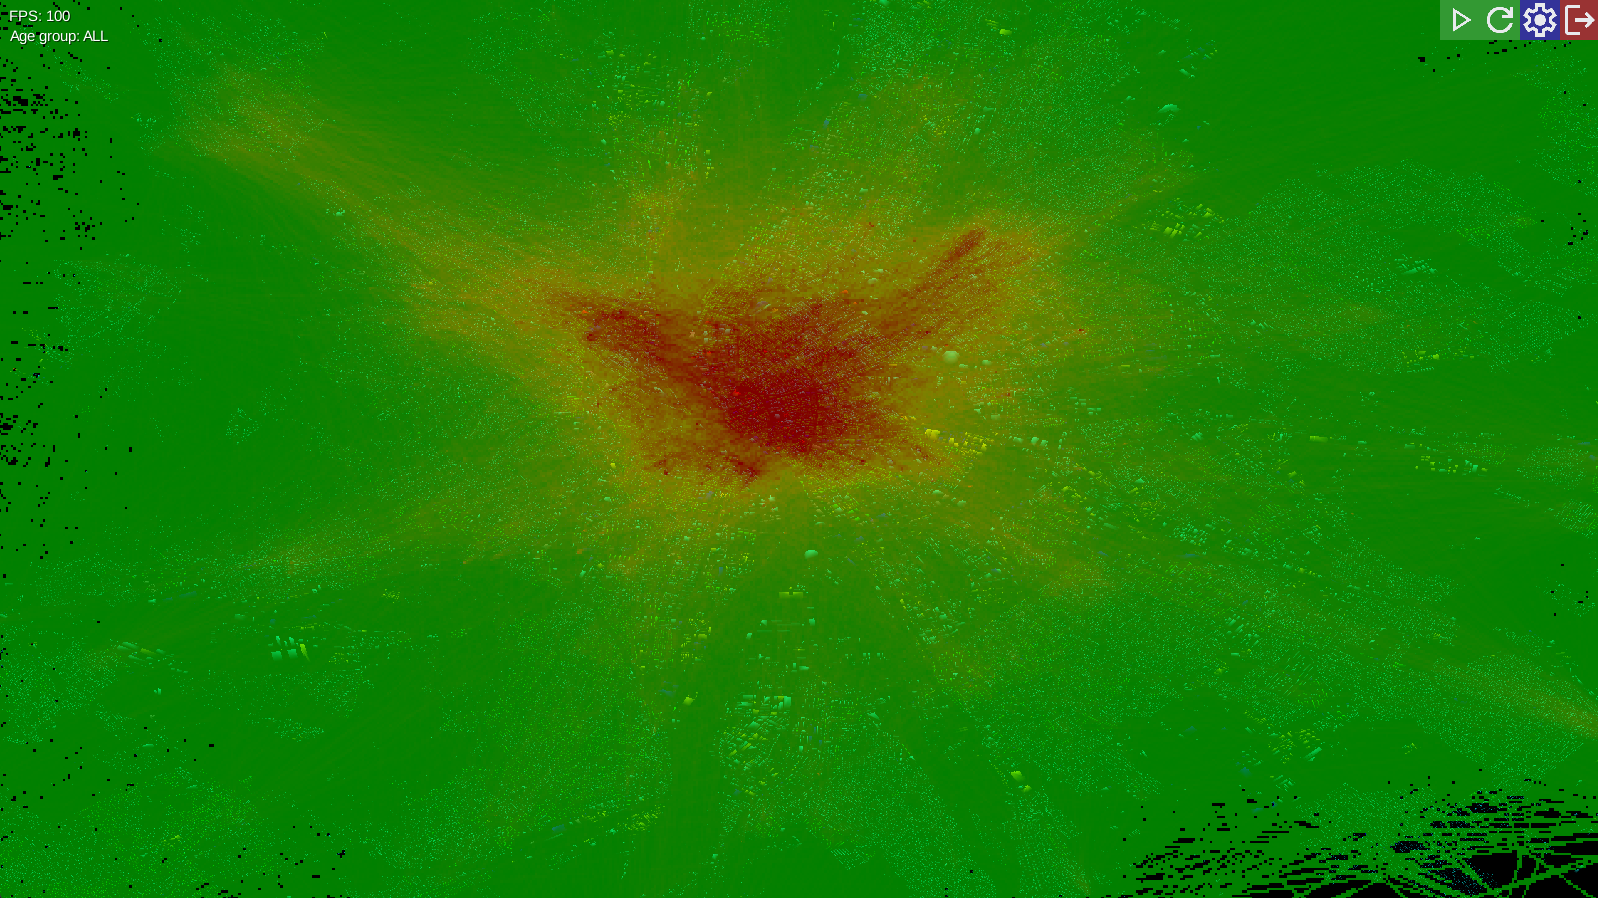
\includegraphics[width=110mm, keepaspectratio]{images/heatmap_50000.png}
    \caption{Heatmap using 50000 agents, see~\ref{perftesting-heatmap}}
\end{figure}

\label{age-groups}
\begin{figure}[!h]
    \centering
    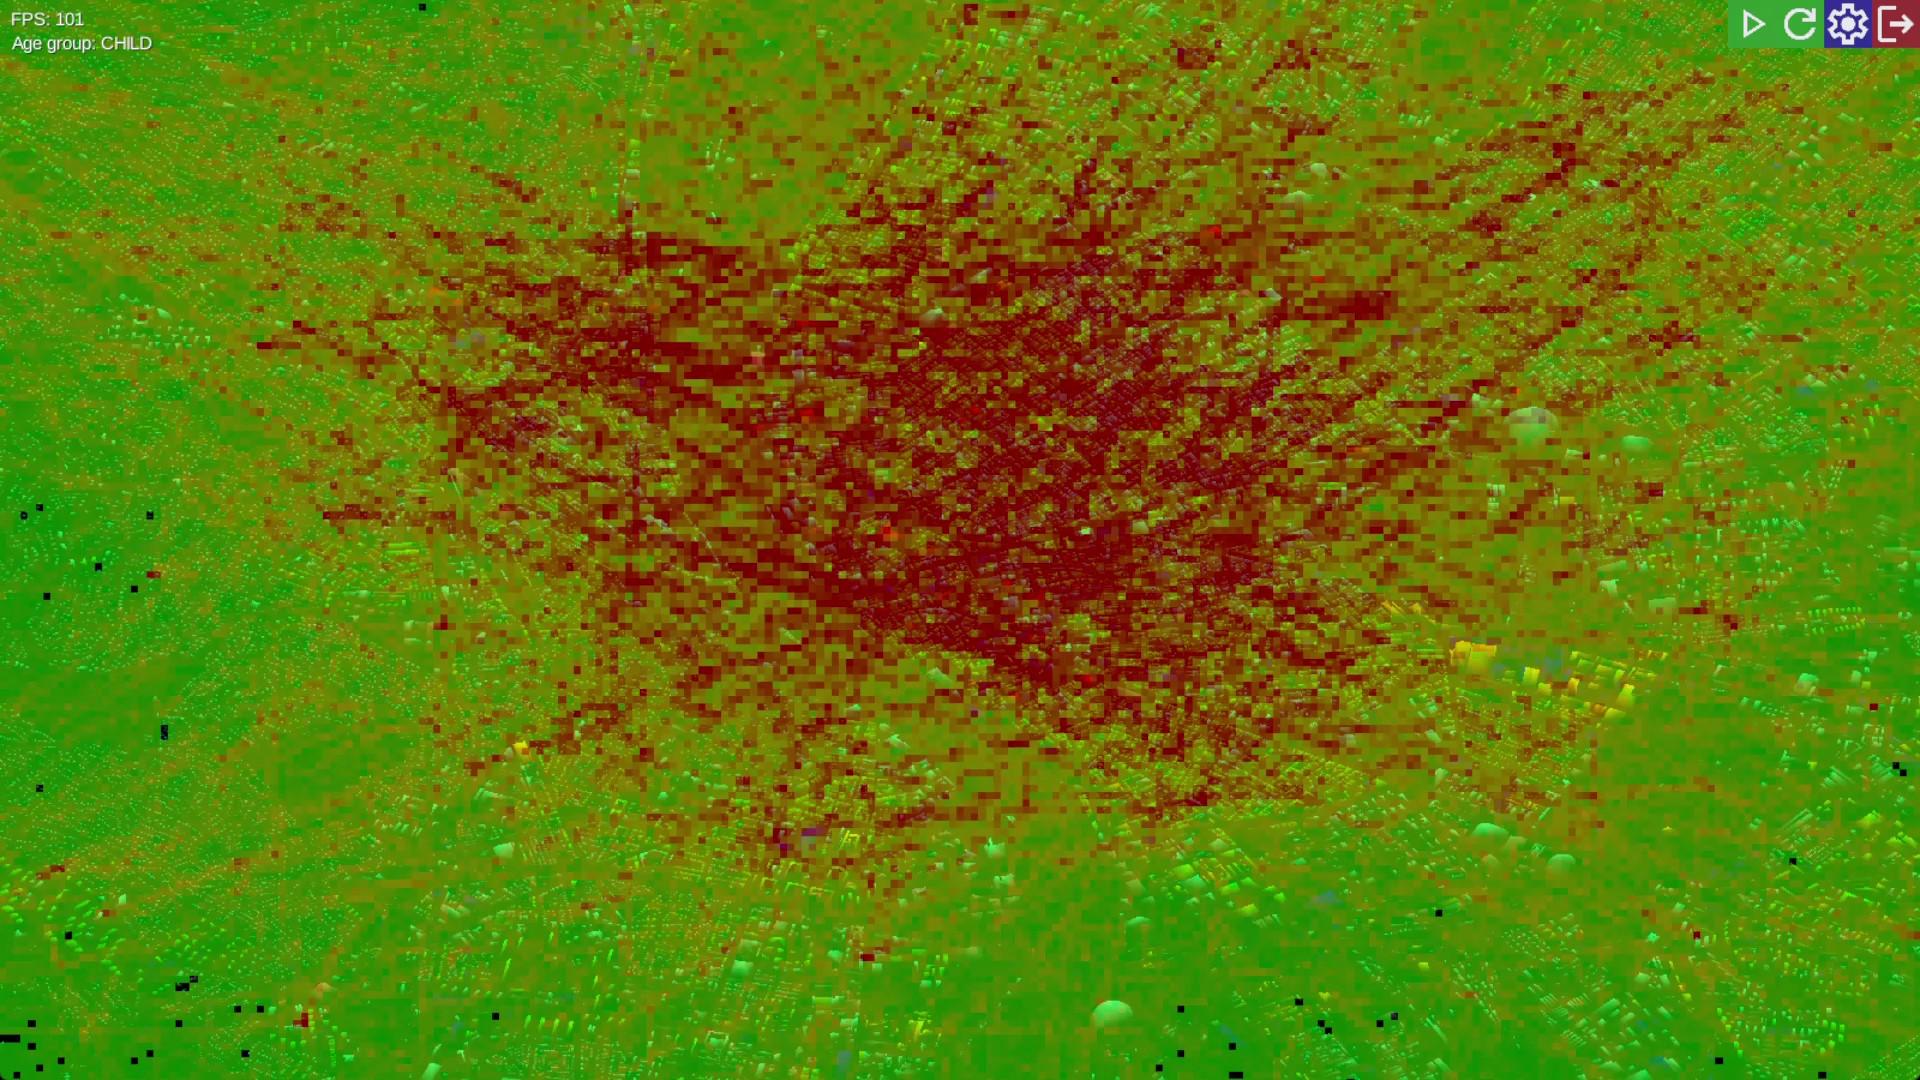
\includegraphics[width=110mm, keepaspectratio]{images/heatmap-children.jpg}
    \caption{Reference simulation heatmap, age group: children}
\end{figure}
\begin{figure}[!h]
    \centering
    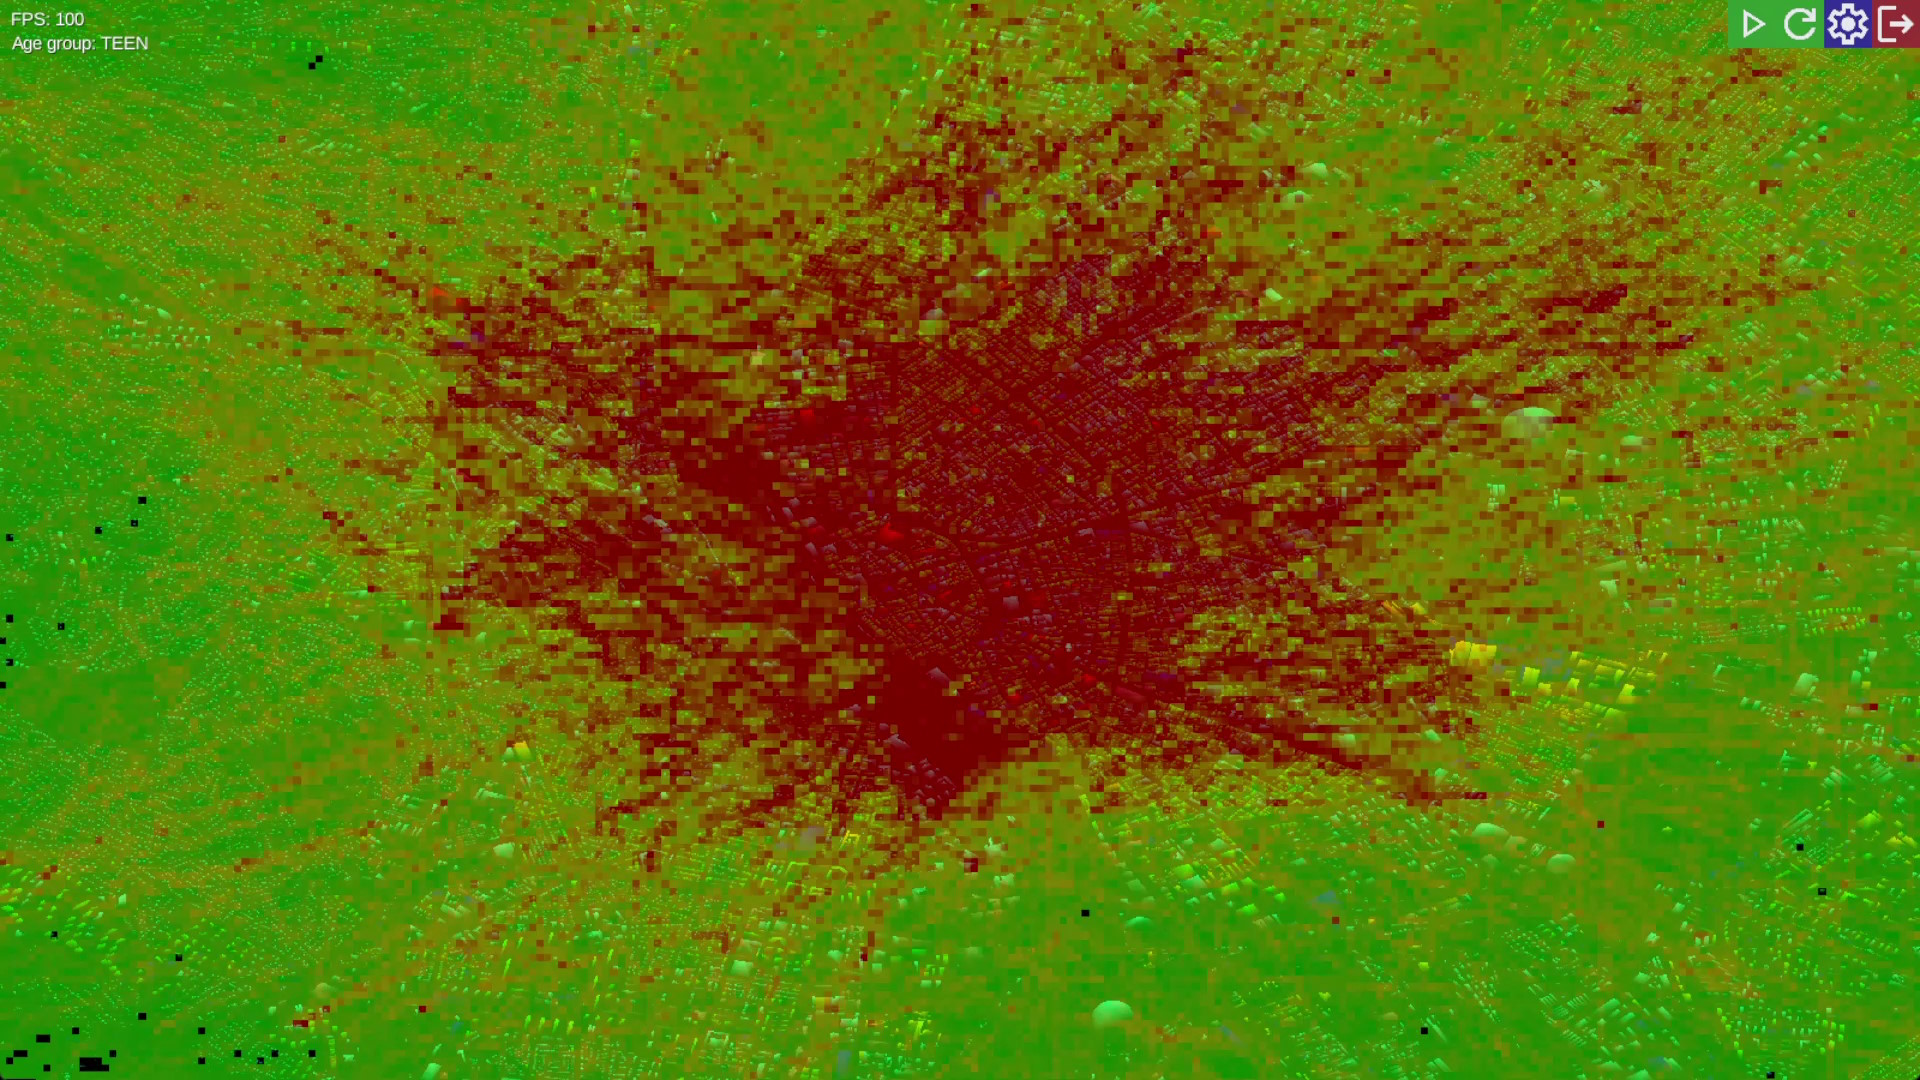
\includegraphics[width=110mm, keepaspectratio]{images/heatmap-teens.jpg}
    \caption{Reference simulation heatmap, age group: teenagers}
\end{figure}
\begin{figure}[!h]
    \centering
    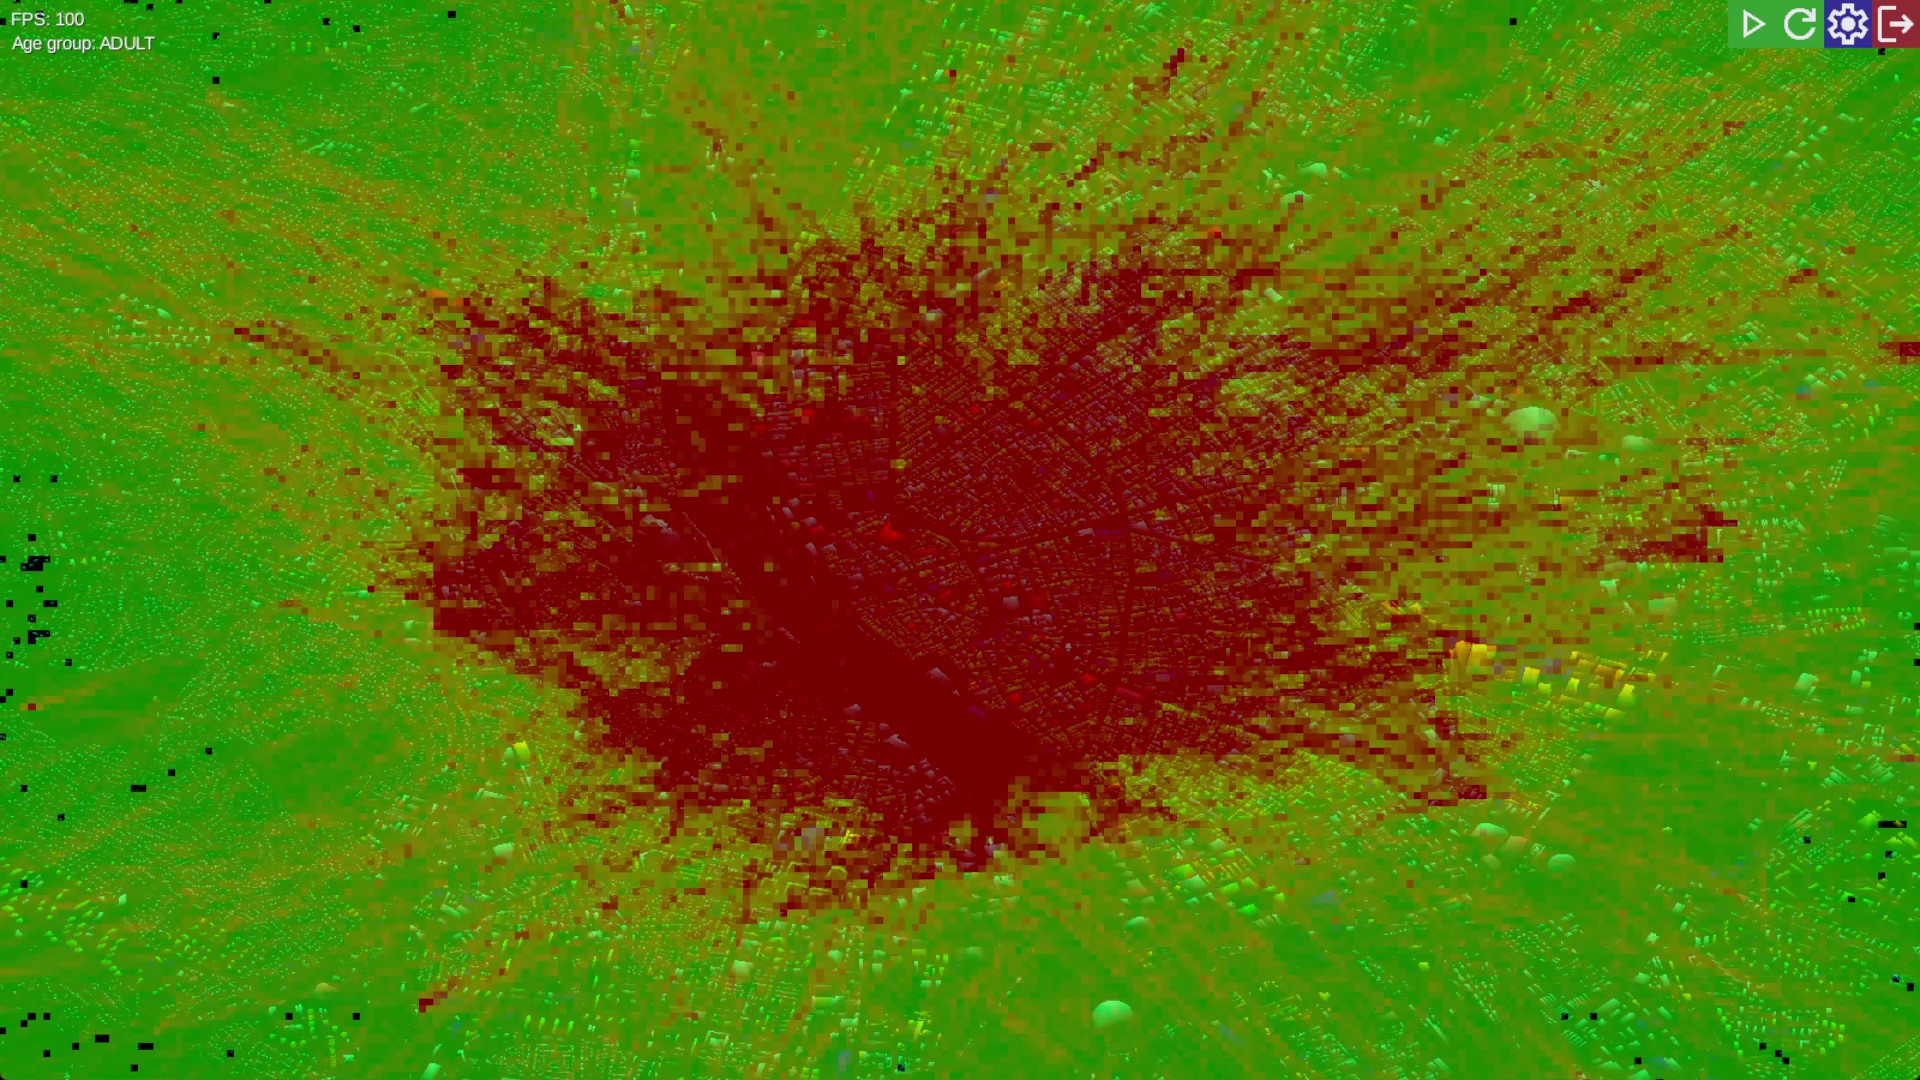
\includegraphics[width=110mm, keepaspectratio]{images/heatmap-adults.jpg}
    \caption{Reference simulation heatmap, age group: adults}
\end{figure}
\begin{figure}[!h]
    \centering
    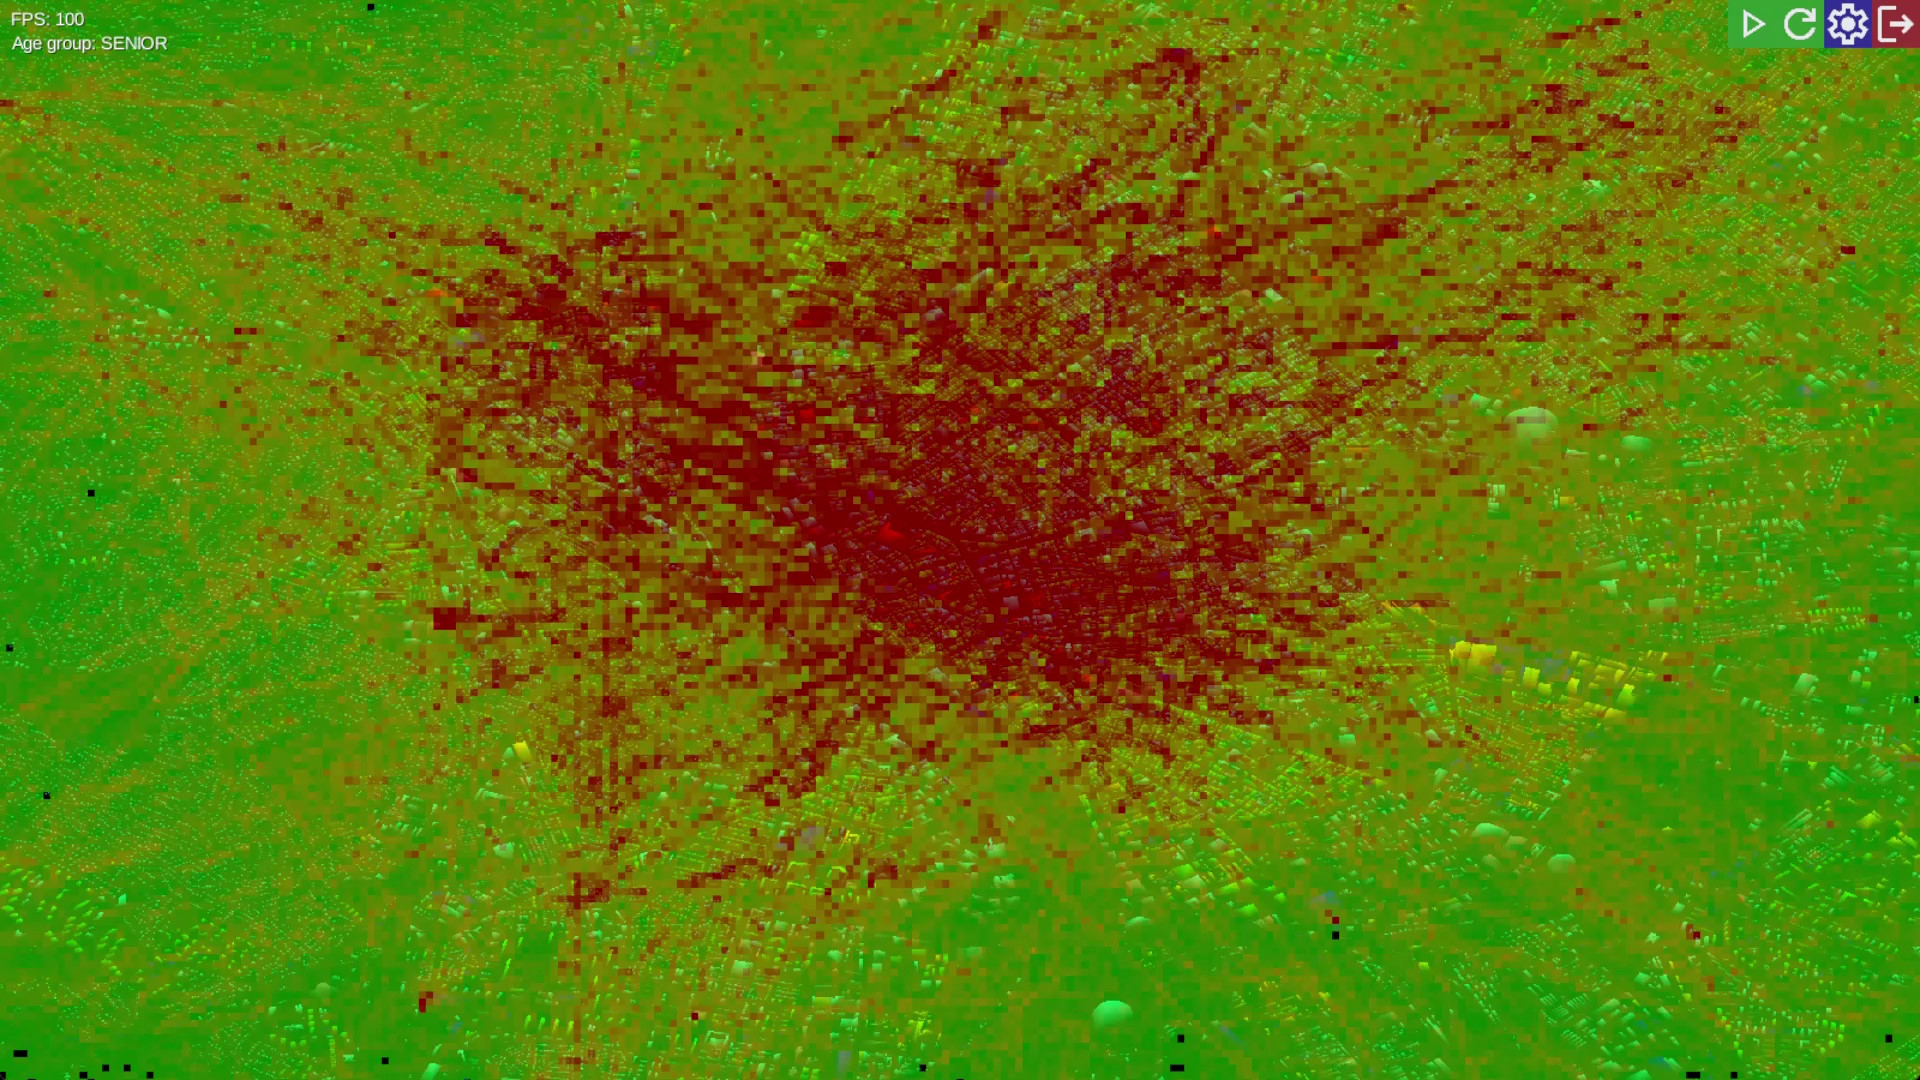
\includegraphics[width=110mm, keepaspectratio]{images/heatmap-seniors.jpg}
    \caption{Reference simulation heatmap, age group: seniors}
\end{figure}